% !TEX root = main.tex
%%%%%%%%%%%%%%%%%%%%%%%%%%%%%%%%%%%%%%%%%%%%%%%%%%%%%%%%%%%%%%%%%%%%%%%%%%%%%%%%
% Time Between Failures Analysis
%%%%%%%%%%%%%%%%%%%%%%%%%%%%%%%%%%%%%%%%%%%%%%%%%%%%%%%%%%%%%%%%%%%%%%%%%%%%%%%%
\section{Time Between Failures Analysis}
\label{section:tbf}

\begin{figure}[bt]
  \begin{center}
    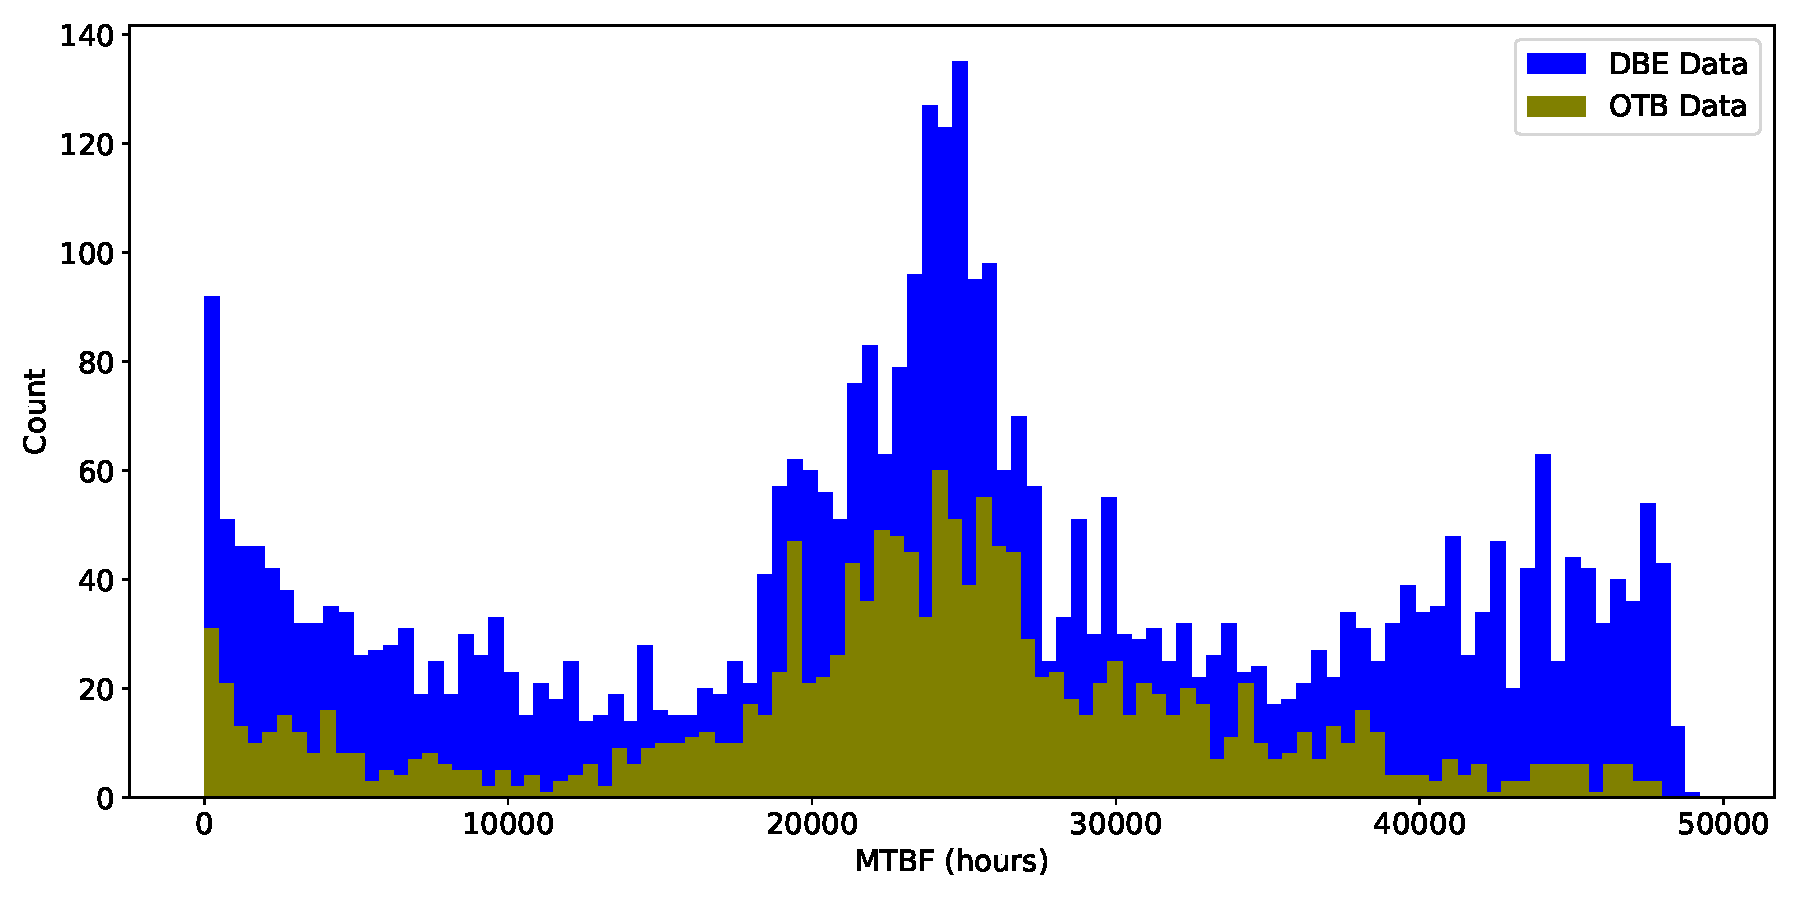
\includegraphics[trim={0 1em 0 1em},clip,width=\columnwidth]{figs/MTBF_GPUwise.pdf}
  \end{center}
  \caption{Distribution of device-level MTBFs due to DBE and OTB failures across all GPUs during the
entire lifetime of the machine. DBE and OTB events are separated for each GPU to distinguish between 
the failure pattern of each event type. Data includes both old and new batch of GPUs with the new ones 
mostly having MTBFs around or less than 3 years.}
  \label{fig:Device_MTBFs}
\end{figure}

Using the cleaned data, we analyze the inter-arrival times between the DBE and OTB events. 
This analysis is done at the device level and at the system level. 
It provides important insights into the reliability of large-scale machines, where the 
failure rate of an individual device is significantly different from the overall reliability
of the machine.  

A histogram of MTBFs measured across GPUs which had at least one failure event is shown 
in Figure~\ref{fig:Device_MTBFs}. This is a practical assessment of device reliabilities 
as opposed to those provided in the device datasheet. The failures are tracked using the
{\em sn} of the GPUs even though a GPU might have been placed at different locations in the 
machine during its lifetime. The time to the first failure on a device is measured by taking
the insert time as the reference point, whereas, a simple difference is taken for subsequent
failures. It can be noticed that MTBFs due to DBE and OTB failures of most GPUs are clustered around 
25,000 hours or 2.8 years. This corresponds to the lifetime of most GPUs in the system after accounting 
for relocations and replacements done in the machine. Almost all of the new batch of GPUs lie below 
the average since most have a lifetime close to 3 years. We point out
that the new batch had a much smaller number of failures than
the old batch as we highlight in the next section.

Apart from the center cluster, many GPUs also have a very 
low MTBF. This failure characteristic is mainly an artifact from
troubleshooting a period of increasing failures in mid to late 2016.
After a GPU experienced an OTB or a DBE a second reboot was attempted at
the same or possibly different location. Usually, but not always, a
second OTB or DBE was generated immediately or possibly after a short
time. When moved to a new location, this generates an artifact in our
data with an unusually short MTBF because we use the {\em insert} time as
a reference for the first failure on a relocated GPU. This drawback is
balanced by the advantage that this way we can discount out of service times
which were frequent particularly during early 2017 as can be seen in
Fig.~\ref{fig:locview}.

On the other end of the spectrum, a noticeable portion of GPUs have very high
MTBFs and their failures are mostly DBEs. These are the GPUs that see continuous operation in the machine 
despite its various episodes and see a single DBE event during their lifetime.
Apart from this, the distribution of MTBF due to DBE events looks very similar to that due 
to OTB events. We also note in Figure~\ref{fig:Device_MTBFs} that the number of recorded 
DBE events is much higher than the OTB events. This highlights the targeted replacement of GPUs 
with OTB events causing a substantial decrease in OTB events.  

%\begin{figure}[bt]
%  \begin{center}
%    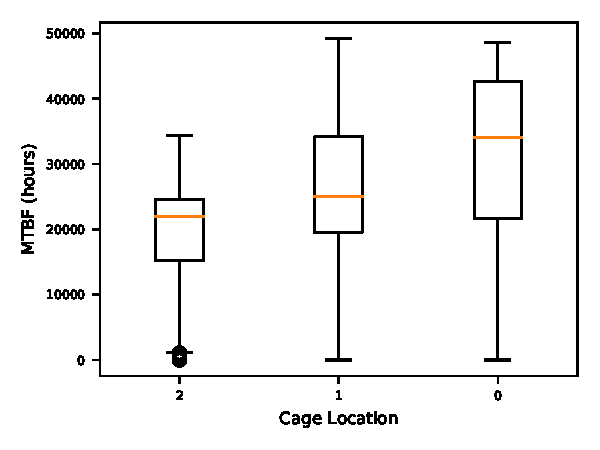
\includegraphics[width=\columnwidth]{figs/MTBF_CageWise.pdf}
%  \end{center}
%  \caption{MTBFs due to either DBEs or OTBs across the GPUs located in different cages.}
%  \label{fig:CageWise_MTBFs}
%\end{figure}

%\fix{Figure~\ref{fig:CageWise_MTBFs} shows temperature effect clearly. Should we move this 
%result to later in the paper?}

\begin{figure}[bt]
  \begin{center}
    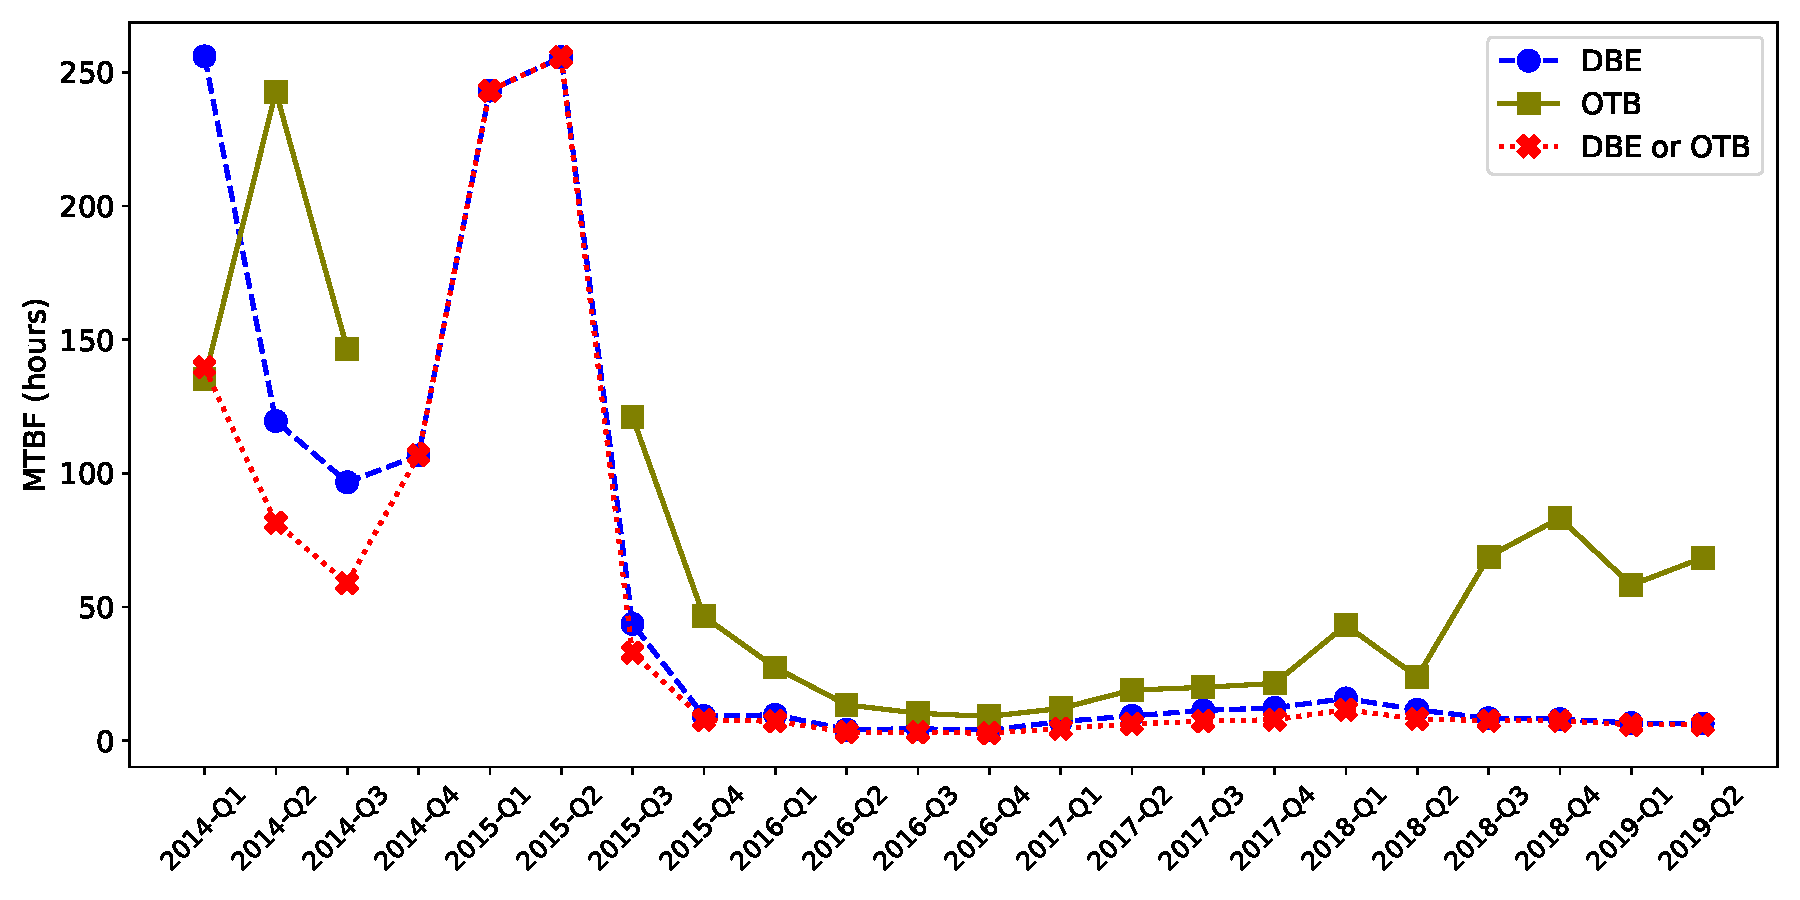
\includegraphics[trim={0 1em 0 1em},clip,width=\columnwidth]{figs/MTBF_quaterly_sys.pdf}
  \end{center}
  \caption{Variation of system-wide MTBF over the lifetime of the machine. System MTBF is calculated over 
three month periods to understand the various episodes of the machine. The three month periods are 
referred to as quarters, i.e., January through March is Q1, and so on. Most GPU replacements started taking 
place at the end of 2016-Q4 and were completed before 2018-Q1. DBE and OTB events are 
considered independently as well as together to represent failures occurring on the machine.}
  \label{fig:MTBF_sys}
\end{figure}

Now we turn to a system-wide MTBF analysis. Most high-performance
computing applications, especially on leadership computing
systems such as Titan, use a large fraction of the entire machine in parallel.  
In the following analysis, failures occurring across all GPUs are consolidated and time between failures
is calculated. The old and new GPUs are all considered. At any given time, only a fixed number of GPUs
is in the system so any variation in time-between-failures is due to individual device reliabilities.

That said, a single MTBF number does not give an accurate picture of this machine.
With many GPU relocations and replacements across the machine over its lifetime, it is 
best to consider the variability of MTBF across fixed periods. Here, we calculate 
the mean of quarterly (three months) time-between-failures. Figure~\ref{fig:MTBF_sys}
shows the considerable change in system-wide MTBF from one period to another. 
We can see that MTBF tells the different phases that occurred on the machine. 
Relatively high MTBFs are seen before 2015-Q4, with some quarters not having any OTB events 
and overall MTBF being determined solely by DBE events. During this
phase, we see some MTBF variation from quarter to quarter, but
generally, the system MTBF remains higher than one day (33 hours) and reaches as high
as 10 days in one instance. An alarming drop in the system MTBF to less than a day, (7.7 hours), is observed in 2015-Q4.
A consistent drop in system-wide MTBF is observed starting from 2015-Q2 until 2016-Q4. 
The corresponding increase in the number of failures during this phase can be seen in Figure~\ref{fig:NumFails_sys},
with a peak in 2016-Q4. The usability of the machine comes into
question with such low MTBFs and it eventually triggered 
a phase of installing new GPUs in the machine.

When GPU replacements start to take place in late 
2016, it triggers a slight increase in MTBF. However, this change only lasts until 2018-Q1, when we see another 
downward trend of system MTBF. Incidentally, 2018-Q1 also marks the completion of all GPU replacements. 
So the upward trend noted in the period from 2016-Q4 to 2018-Q1 is
likely due to phased replacements, each time a portion of the machine 
being unavailable, thus having a smaller number of GPUs than the full
machine in operation. 
%\fix{need to verify how long the replacement took}
There is not definitive way to incorporate this unavailability of the
machine into MTBF analysis, unless we know how the down times were scheduled.
The lowest MTBF obtained in 2016-Q4 is 2.7 hours, with subsequent periods having the 
lowest MTBF of 5.9 hours. With system MTBF less than a day, even slight variations in MTBF make it 
difficult to reliably run applications despite using failure recovery approaches such as checkpoint restart, 
as discussed later on in Section~\ref{section:discussion}. 

\begin{figure}[bt]
  \begin{center}
    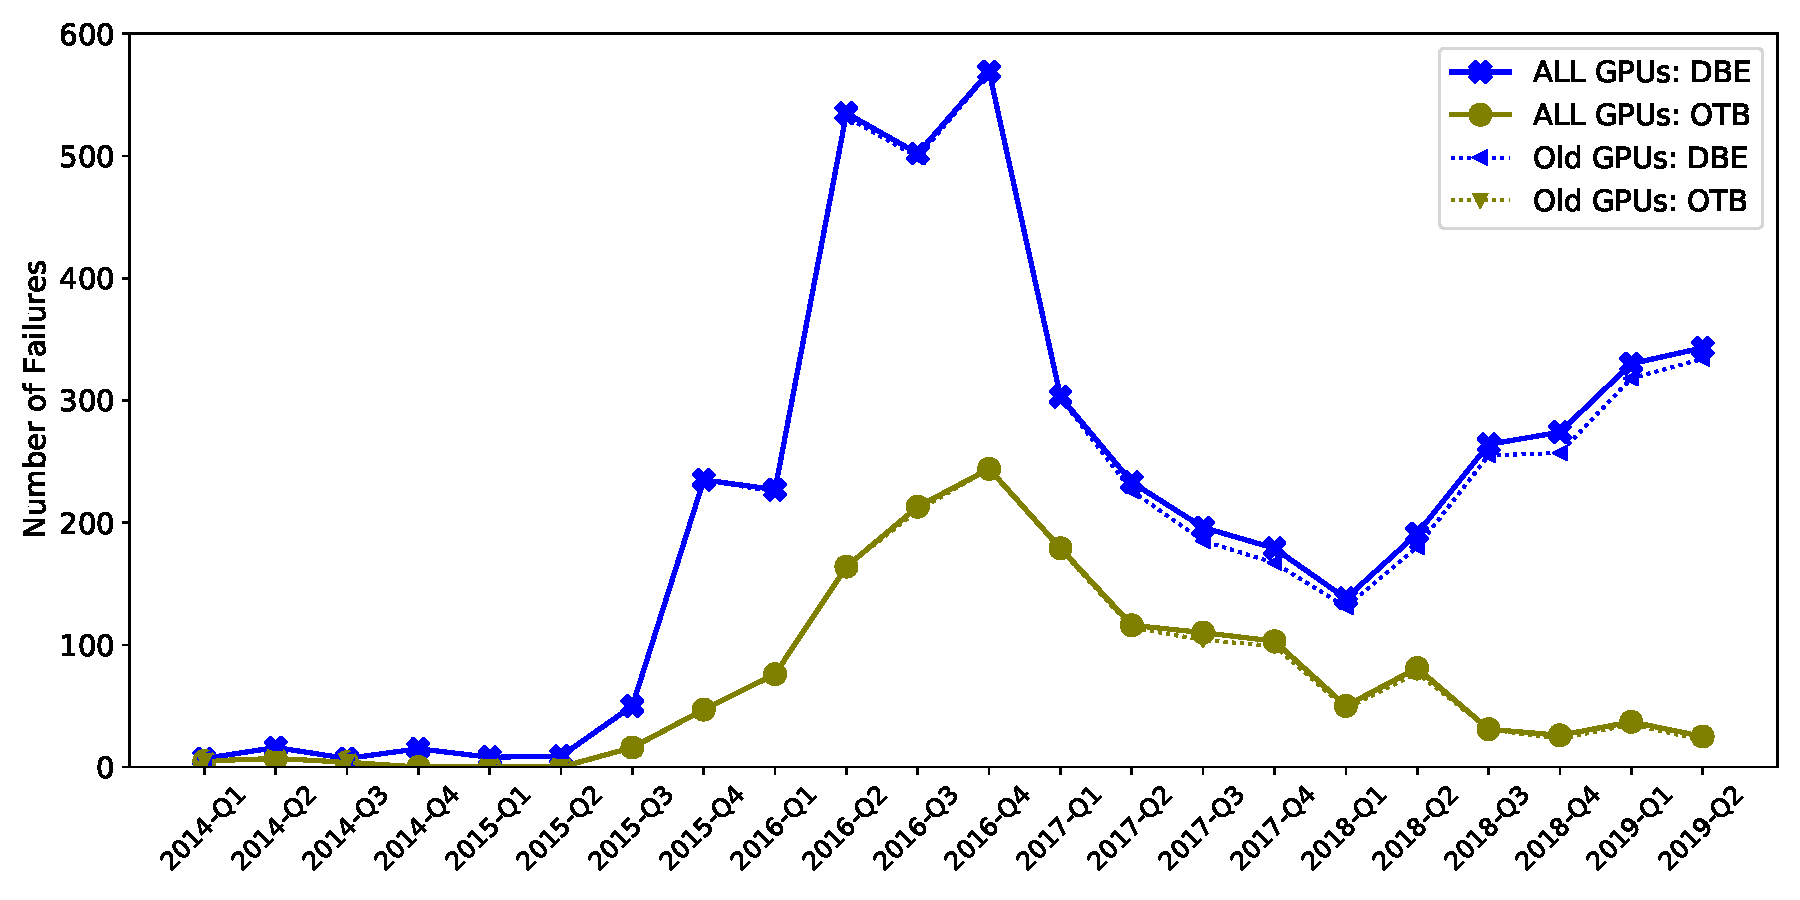
\includegraphics[trim={0 1em 0 1em},clip,width=\columnwidth]{figs/NumFailures_Quarterly_newOld.pdf}
  \end{center}
  \caption{The number of DBE and OTB failures observed over the lifetime of the machine.
A distinction is made between failures on old GPUs to highlight the number
of failures on the newer GPUs. The peak failures are seen in 2016-Q4 (813 failures), 
which marks the commencement of major replacement of GPUs in the machine.}
  \label{fig:NumFails_sys}
\end{figure}

\begin{figure}[bt]
  \begin{center}
    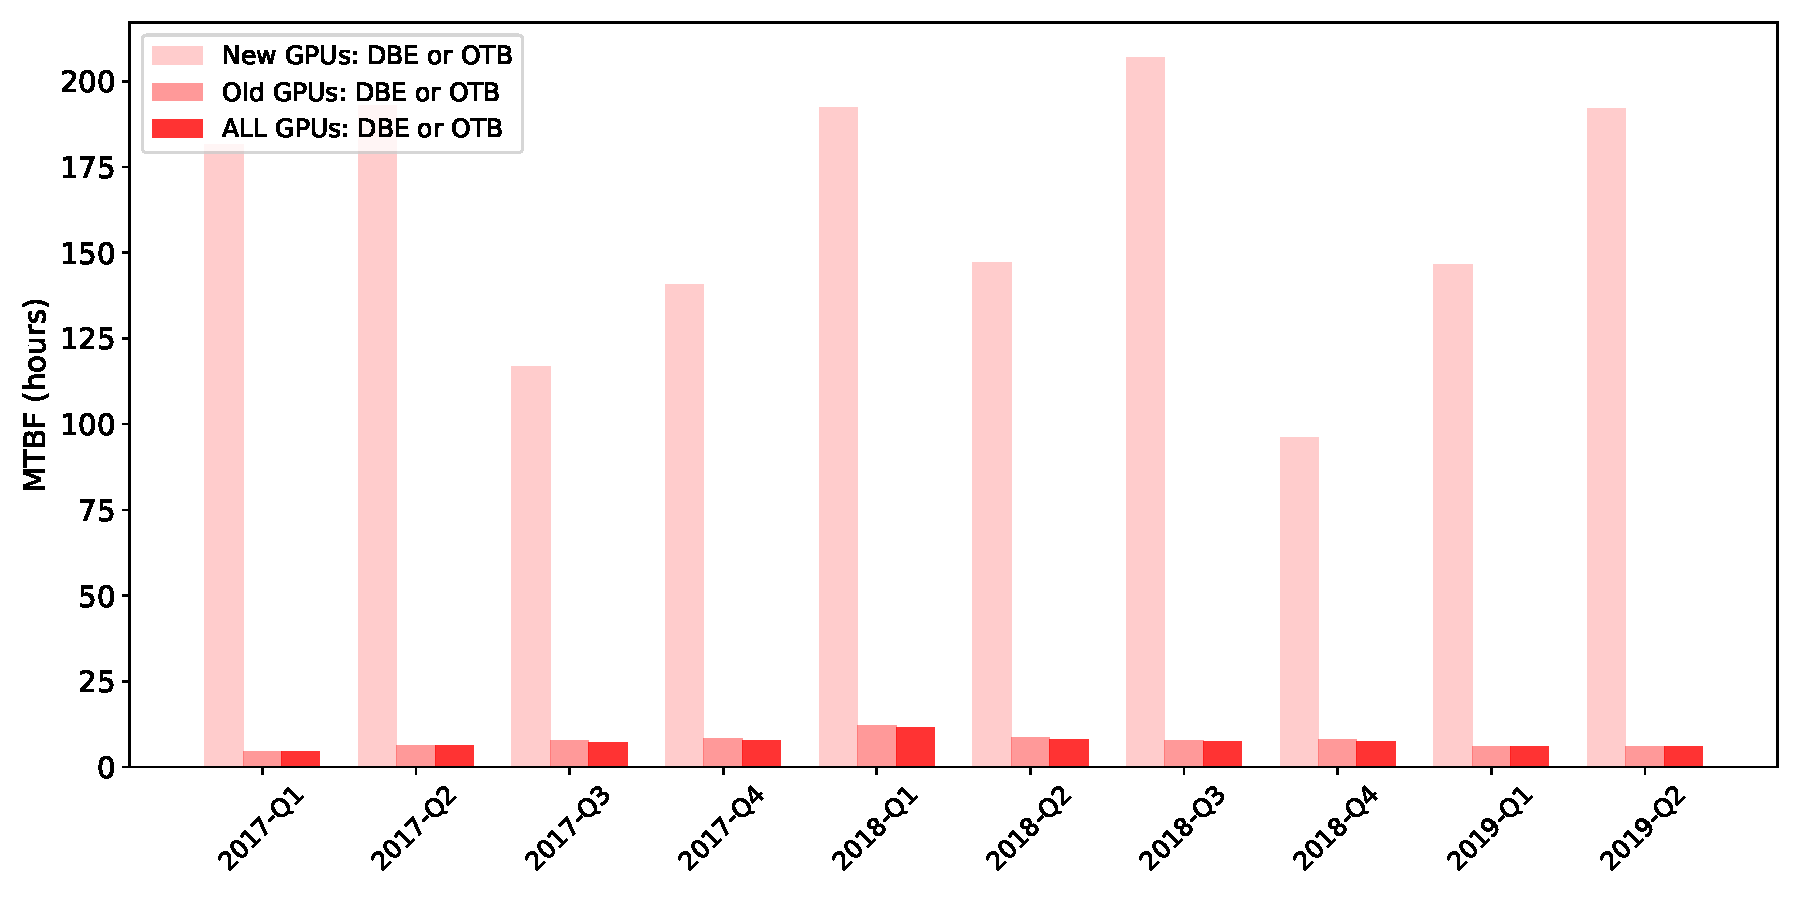
\includegraphics[trim={0 1em 0 1em},clip,width=\columnwidth]{figs/MTBF_quaterly_sys_NewOldALL.pdf}
  \end{center}
  \caption{Variation of system-wide MTBF across hypothetical new and
    old partitions of the machine after a substantial number of new GPUs
were put in service.
DBE and OTB events both determine the MTBF.
Results highlight the difference in reliability for jobs using the new GPUs as compared to old GPUs,
as well as now MTBF is driven by the weaker old partition.}
  \label{fig:MTBF_sys_NewOld}
\end{figure}
We also separate the DBE and OTB failures in this analysis. After the
2017 replacement of many GPUs, there is a drastic increase in
mean-time-between OTB failures, which is also evident in a reduction of OTB failures in Figure~\ref{fig:NumFails_sys}.
However, the system MTBF is determined by the weakest link and here the occurrence of DBE events tends to dictate it.
Even though the replacements helped to increase the MTBF due to DBE events, the overall system 
reliability is dictated by the components with the most age in the
system. There is a re-emergence of an upward trend towards 
the end in DBE failures in Figure~\ref{fig:NumFails_sys}, which
appears to be due to older GPUs in the system. 

To better understand the difference in reliability of newer and old portions of the machine, 
Figure~\ref{fig:MTBF_sys_NewOld} shows the drastic difference in system MTBF measured in two hypothetical
partitions of the machine starting from the time when the majority of GPU replacements have been completed. 
The new partition of the machine has a 12X better MTBF than the older
partition.

For example, in 2018-Q4, the old partition MTBF is about 7.9 hours,
whereas the newer partition is 96 hours (4 days). The implications of such a huge disparity on applications running on the 
system are discussed in
Section~\ref{section:discussion}. Moreover, while the old partition is
smaller than the new partition, the old partition drives the overall reliability of
the machine.
